\documentclass[11pt]{article}
\usepackage{geometry}                % See geometry.pdf to learn the layout options. There are lots.
\geometry{letterpaper}                   % ... or a4paper or a5paper or ... 
%\geometry{landscape}                % Activate for for rotated page geometry
%\usepackage[parfill]{parskip}    % Activate to begin paragraphs with an empty line rather than an indent
\usepackage{graphicx}
\usepackage{amssymb}
\usepackage{amsmath}
\usepackage{epstopdf}
\usepackage{hyperref}
\DeclareGraphicsRule{.tif}{png}{.png}{`convert #1 `dirname #1`/`basename #1 .tif`.png}


\graphicspath{
{/Users/Andy/Cruises_Research/Analysis/Andy_Pickering/eq14_patch_gamma/figures/}
{/Users/Andy/Cruises_Research/Analysis/Andy_Pickering/eq14_patch_gamma/figures/chi_eps_profiles_10profavgs/zsm10m_fmax7Hz_respcorr0_fc_99hz_gamma20_nfft_128_screen_chi_1/}
}

\title{Summary of $\chi$pod Chameleon EQ14 Analysis}
\author{Andy Pickering}
%\date{}                                           % Activate to display a given date or no date



\begin{document}
\maketitle

\tableofcontents
\newpage


%~~~~~~~~~~~~~~~~~~~~~~~~~~~~~~~~~~~~~~~~
\section{Overview}
%~~~~~~~~~~~~~~~~~~~~~~~~~~~~~~~~~~~~~~~~

\begin{itemize}

\item This document is an attempt to provide an overview/summary of what i've found in my $\chi$pod analysis. 

\item The motivation/goal for all this work is to show if and how well the CTD-$\chi$pod method works for estimating $\chi$,$\epsilon$, $K_T$, etc from fast temperature profiles. The idea is to deploy $\chi$pods on regular CTD casts on WOCE/CLIVAR cruises etc. to making mixing measurements.

\item Before dealing with all the issues with the CTD deployments (depth loops, entraining water, rosette-induced turbulence etc.), I wanted to verify that the method itself worked w/out these complications. 

\item The Chameleon microstructure profiler has both thermistor and shear probes, so this seemed like an ideal way to test the method. I would apply the $\chi$pod method to the chameleon thermistor data only ($\chi_{\chi},\epsilon_{\chi}$), and compare to the 'true' results computed using the shear probes ($\chi$,$\epsilon$).

\item I found that basically the estimates of $\chi$ agreed, but $\epsilon_{\chi}$ was about an order of magnitude smaller than $\epsilon$ (Figure \ref{chi_overview},\ref{eps_overview},\ref{chamVschi}).

\item The $\chi$pod method requires assuming a mixing efficiency, and uses the normal assumption that $\gamma=0.2$. I computed gamma from the chameleon data (formula) and found that it was about an order of magnitude smaller than 0.2; hence the low epsilon estimates. 

\item Is gamma really different here? Am I calculating it wrong? What does gamma mean? Sasha found something similar previously in EQ08 and other Chameleon datasets, gives me a little more confidence that i'm not doing something obviously wrong..

\item One idea was that we should be computing gamma over patches, and it's meaningless outside of patches. Previous work has found gamma is close to 0.2 . So I tried computing patches and gamma. This can be a whole other can of worms (lots of choices to make in how to identify patches, compute N2, Tz etc), but I found I could get gammas close to 0.2 .  And on a point-by-point basis, $\epsilon_{\chi}$ agreed better with $\epsilon_{\chi}$. But then we have much fewer data points... 

\item Looked at whether averaging multiple profiles agreed better. Doesn't seem to make epsilon agree. However, gamma computed from average quanitites is closer to 0.2?

\item So, is gamma really small here, or am I just computing it wrong? Look at other locations/regimes?

\end{itemize}




\clearpage
%~~~~~~~~~~~~~~~~~~~~~~~~~~~~~~~~~~~~~~~~
\section{Data and Processing}
%~~~~~~~~~~~~~~~~~~~~~~~~~~~~~~~~~~~~~~~~

\begin{itemize}

\item \verb+ComputeChi_Chameleon_Eq14.m+ : Applies $\chi$pod method to Chameleon profiles from EQ14.

\item Sally shared w/ me Chameleon data that she and Jim processed. I ended up re-processing it using a smaller fmax (7Hz) because it looked like the thermistor spectra rolled off much lower than the assumed 32Hz.

\item \verb+Make_Overview_Plots.m+ Makes almost all the figures in this document.

\end{itemize}




\clearpage
%~~~~~~~~~~~~~~~~~~~~~~~~~~~~~~~~~~~~~~~~
\section{?}
%~~~~~~~~~~~~~~~~~~~~~~~~~~~~~~~~~~~~~~~~

% misc_Appr14.m
\begin{figure}[htbp]
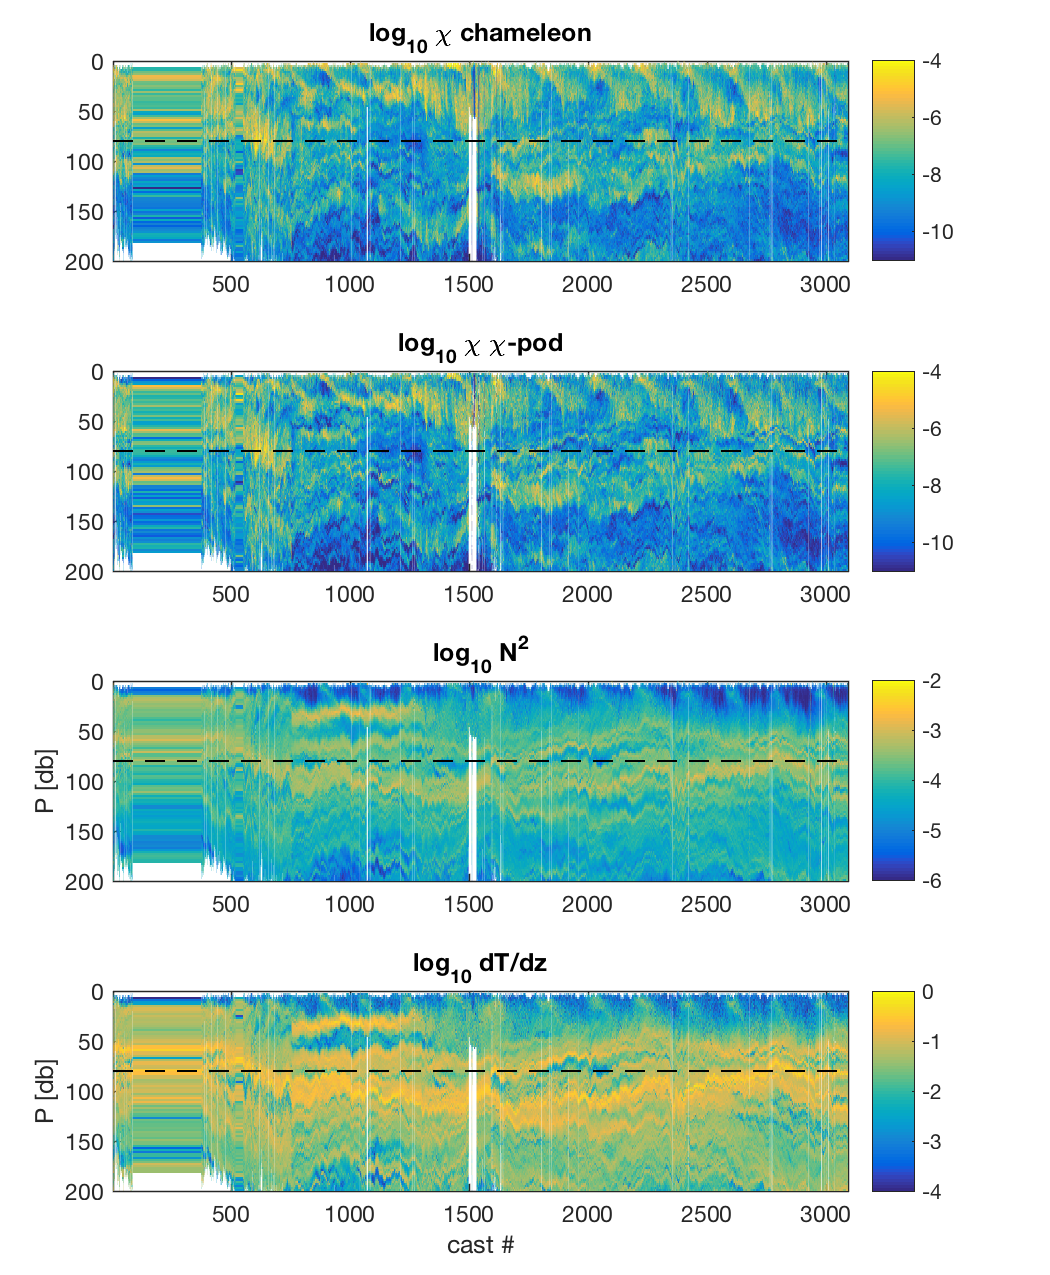
\includegraphics[scale=0.8]{eq14_Pcolor_BothChi_N2_Tz_zsmooth_10_2mbin_screen_chi_1.png}
\caption{Comparison of $\chi$ from chameleon method and chi-pod method, for EQ14 chameleon profiles. Each profile was averaged in 2m bins.  Horizontal line at 80m shows region excluded in further analysis because it contains near-surface convection.}
\label{chi_overview}
\end{figure}

\begin{figure}[htbp]
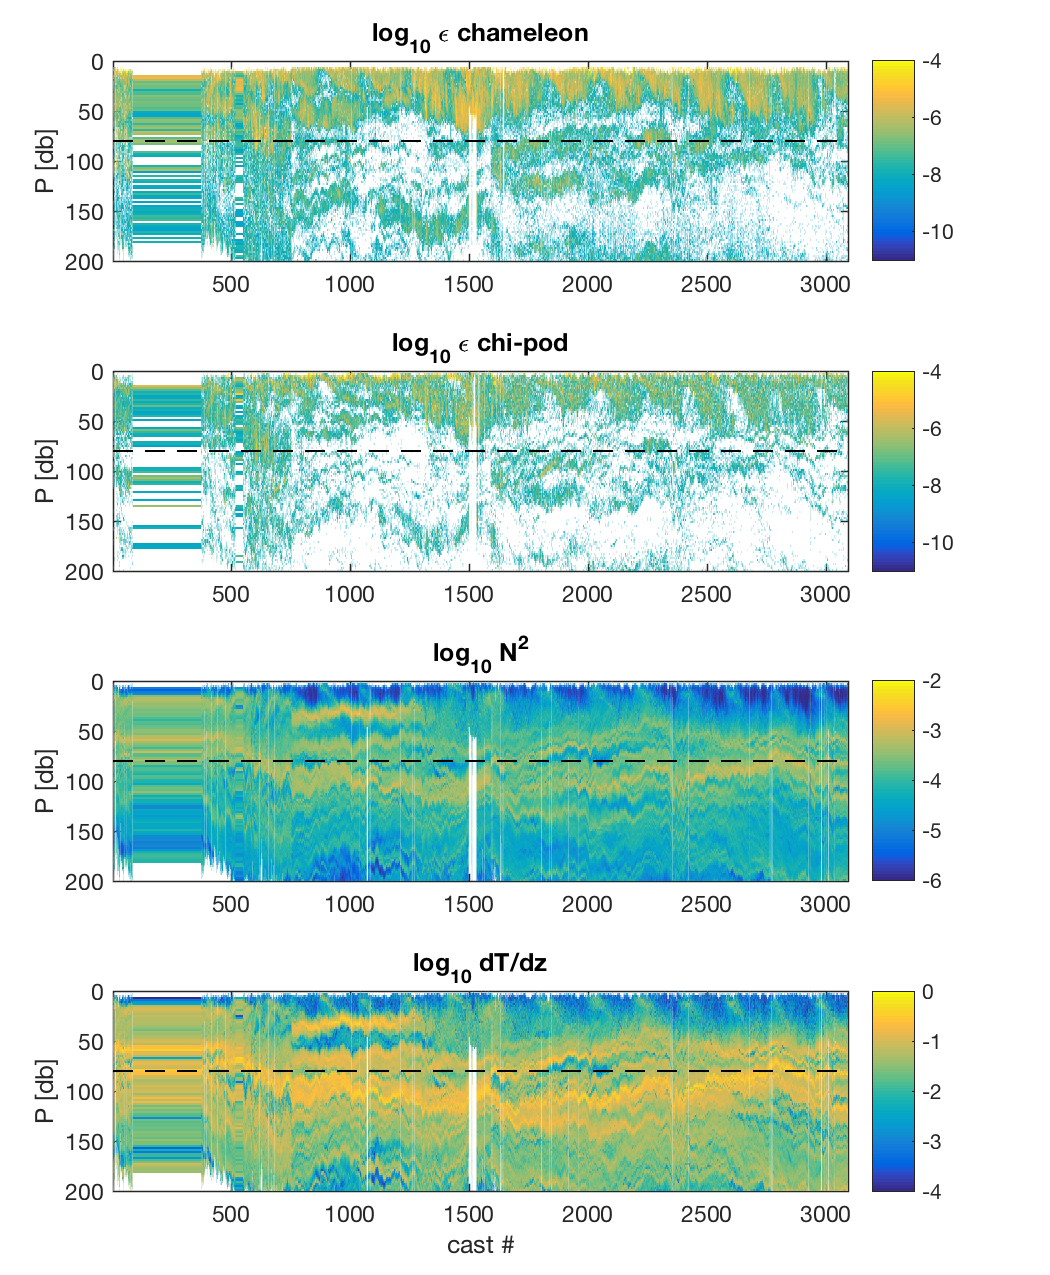
\includegraphics[scale=0.8]{eq14_Pcolor_BothEps_N2_Tz_zsmooth_10_2mbin_screen_chi_1.png}
\caption{Comparison of $\epsilon$ from chameleon method and chi-pod method, for EQ14 chameleon profiles. Each profile was averaged in 2m bins.  Values of $\epsion$ below chameleon noise floor (-8.5) have been nan'd out. Horizontal line at 80m shows region excluded in further analysis because it contains near-surface convection.}
\label{eps_overview}
\end{figure}



%  plot of $\chi$pod vs cham for chi and eps
\begin{figure}[htbp]
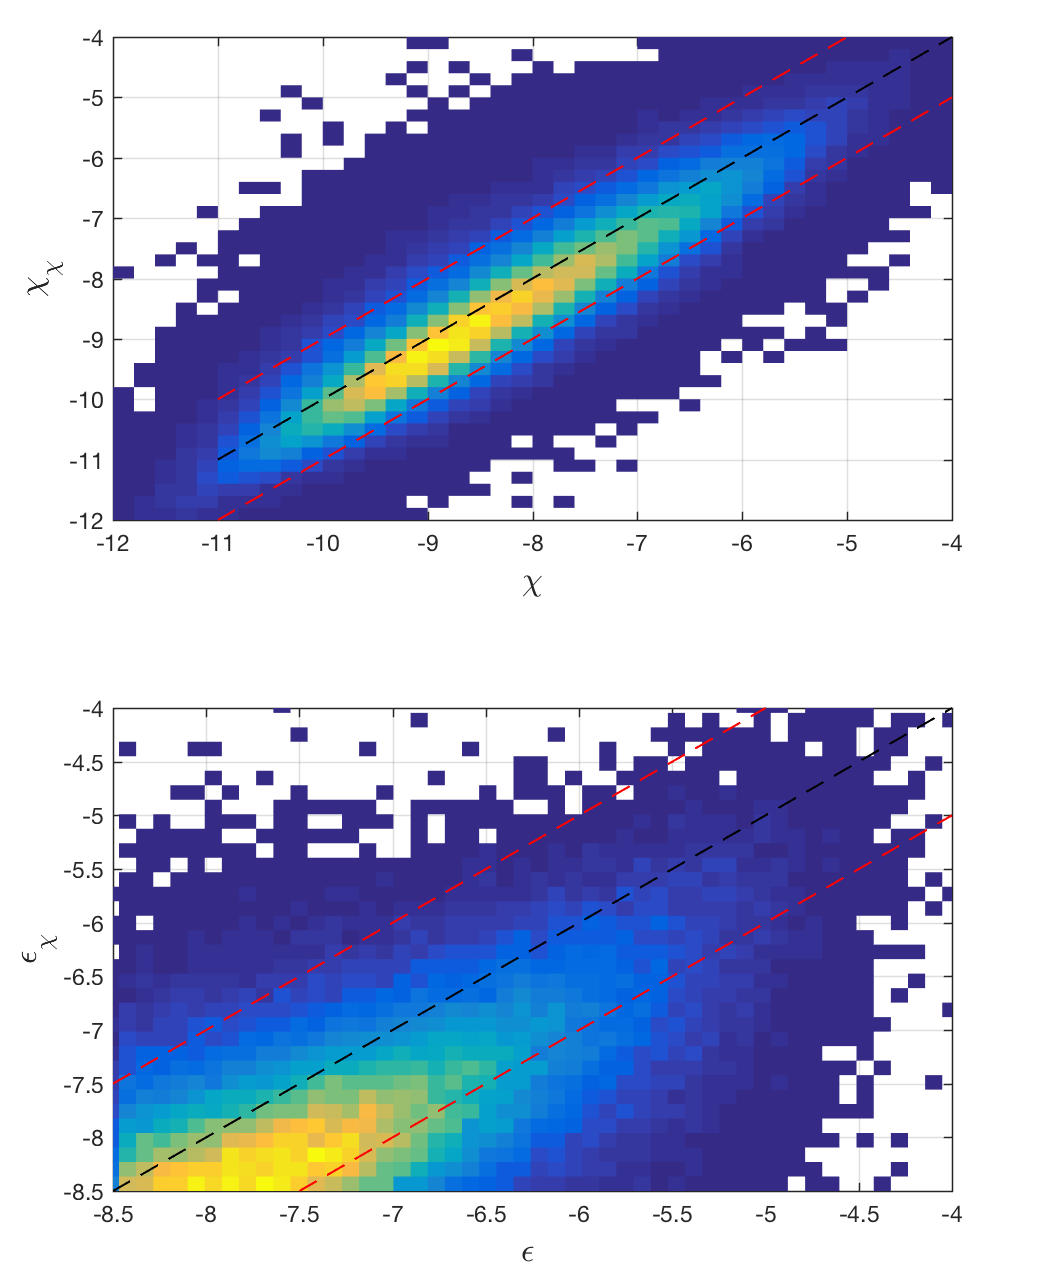
\includegraphics[scale=0.8]{eq14_chamVschipod_10_2mbin_screen_chi_1.png}
\caption{Comparison of $\chi$ $\epsilon$ from chameleon method and chi-pod method, for EQ14 chameleon profiles. Each profile was averaged in 2m bins.  Values of $\epsion$ below chameleon noise floor (-8.5) have been naned out. Black line is 1:1, red lines are $+/-$ order of magnitude. Only data below 80m is used.}
\label{chamVschi}
\end{figure}




\clearpage
%~~~~~~~~~~~~~~~~~~~~~~~~~~~~~~~~~~~~~~~~
\section{Comparing individual estimates of $\epsilon$}
%~~~~~~~~~~~~~~~~~~~~~~~~~~~~~~~~~~~~~~~~

\begin{figure}[htbp]
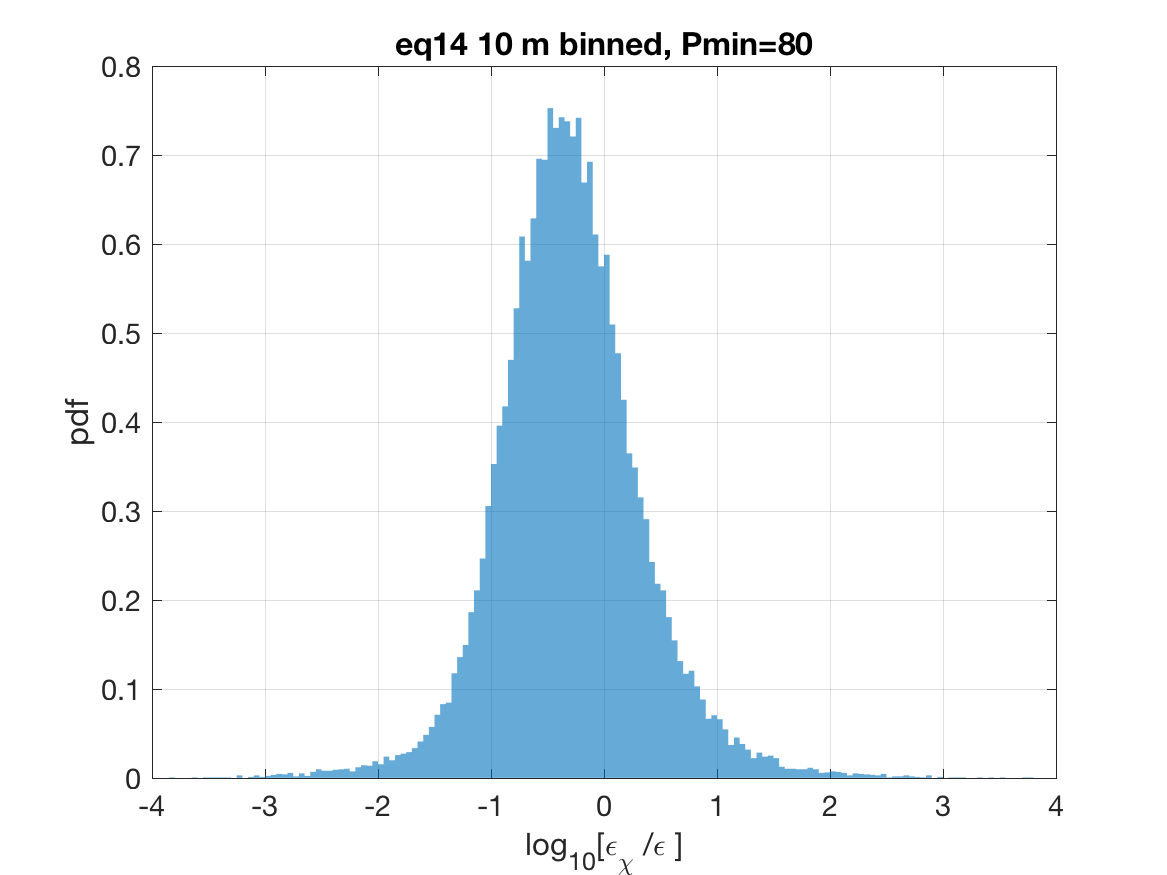
\includegraphics[scale=0.8]{eq14_10mbinned_eps_ratios_Pmin80_screen_chi_1.png}
\caption{EQ14: Histogram of the ratio of $\epsilon$ estimates from $\chi$pod method to the chameleon values, for $\chi$pod method applied to 1m binned profiles, and applied to just patches. Estimates for each profile were averaged in 10m depth bins.}
\label{epsrathist_eq14}
\end{figure}





\clearpage
%~~~~~~~~~~~~~~~~~~~~~~~~~~~~~~~~~~~~~~~~
\section{Normalized eps vs chi plots}
%~~~~~~~~~~~~~~~~~~~~~~~~~~~~~~~~~~~~~~~~

Assuming that
\begin{equation}
\gamma=\frac{N^2 \chi}{2\epsilon<T_z>^2}
\end{equation}
, plotting [$\chi/t_{z}^{2}$] vs [$\epsilon/N\^2$] should follow a straight line with slope equal to $2\gamma$.


\begin{figure}[htbp]
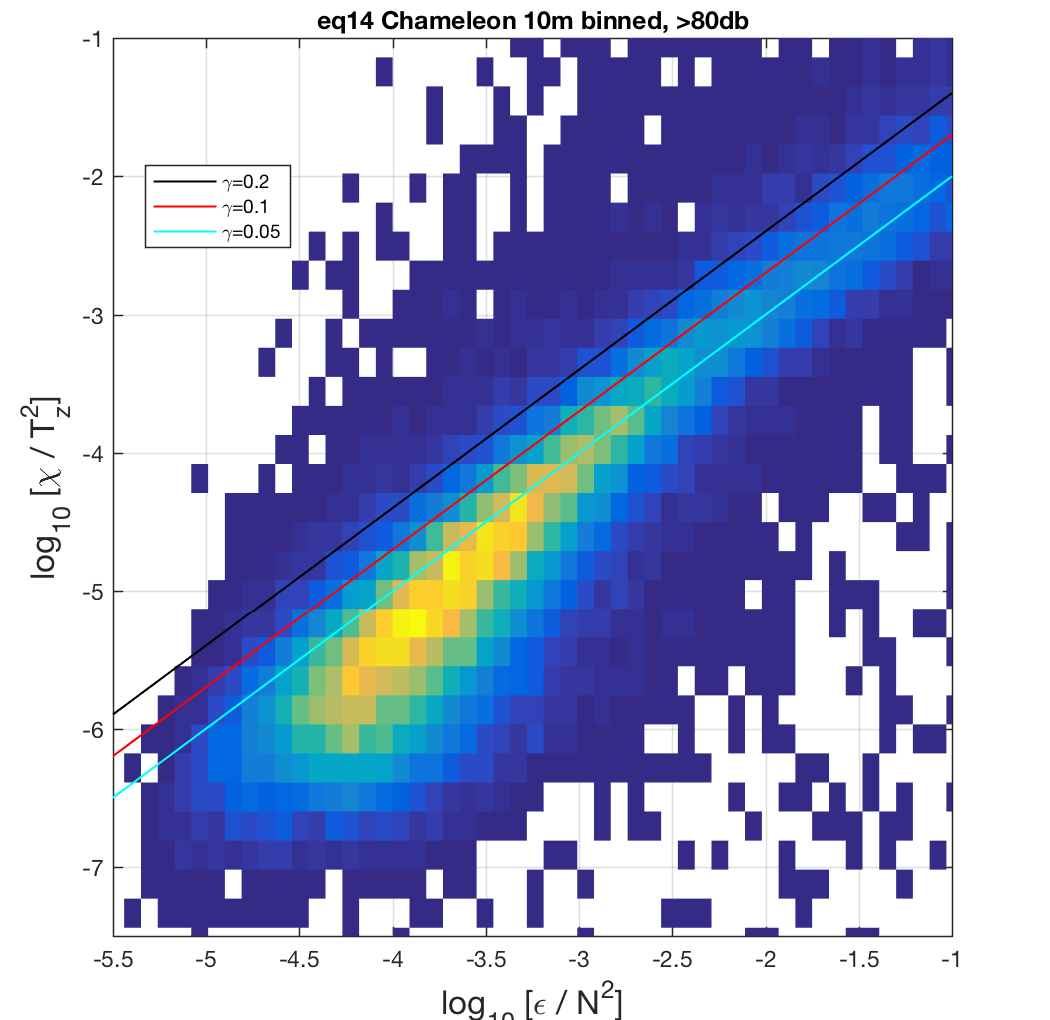
\includegraphics[scale=0.8]{eq14_10mbinned_eps_vs_chi_normalized_Pmin_80.png}
\caption{EQ14: 10m binned  chameleon $\epsilon/N\^2$ vs $\chi/t_{z}^{2}$ for *below 80db*. Lines show different values of $\gamma$. Values of $\epsilon$ below noise floor ($log_{10}\epsilon<-8.5$) are discarded also.}
\label{}
\end{figure}





\clearpage
%~~~~~~~~~~~~~~~~~~~~~~~~~~~~~~~~~~~~~~~~
\section{Averaging many profiles of $\epsilon$}
%~~~~~~~~~~~~~~~~~~~~~~~~~~~~~~~~~~~~~~~~

Figure \ref{prof_avg_ex} shows one example. A folder with many profiles is located at:
\url{https://github.com/OceanMixingGroup/Analysis/tree/master/Andy_Pickering/eq14_patch_gamma/figures/chi_eps_profiles_40profavgs}. %In general, it seems that averaging profiles does not change the comparsion much; $\epsilon_{\chi}$ is still biased low.

\begin{figure}[htbp]
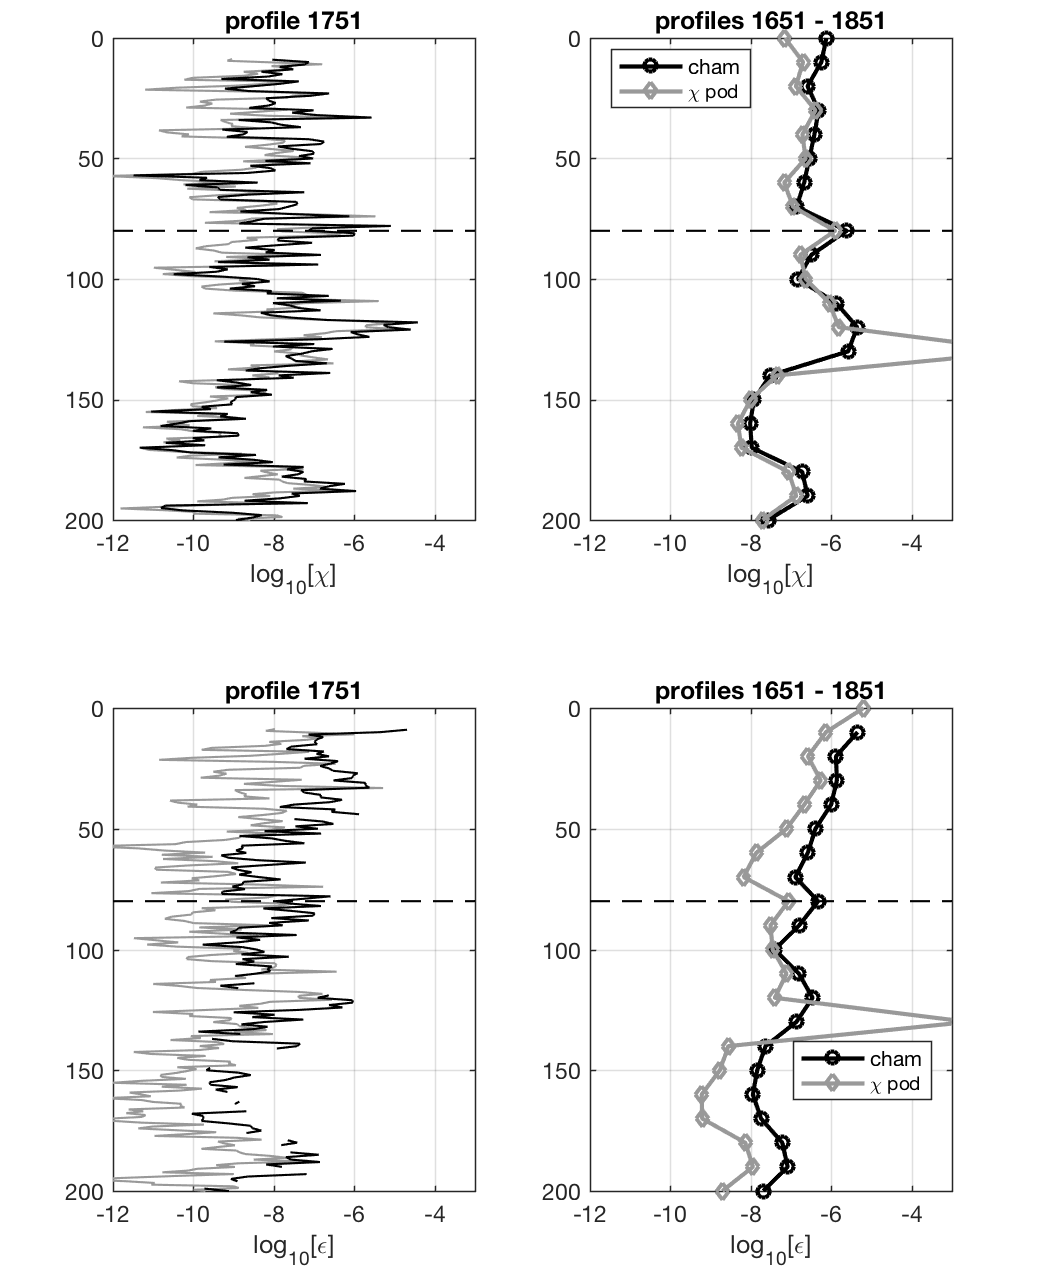
\includegraphics[scale=0.8]{eq14_profile_1751_eps_profiiles_compare.png}
\caption{Example of averaging multiple profiles together. Left panels show a single profile from chamleeon and chi-pod method. Right panels show average of $+/-$ 40 profiles, averaged in 10m depth bins.}
\label{prof_avg_ex}
\end{figure}



I tried making plots of normalized chi vs eps, and scatterplots of chi-pod vs chameleon epsilon, for data averaged across different numbers of profiles. 

\begin{figure}[htbp]
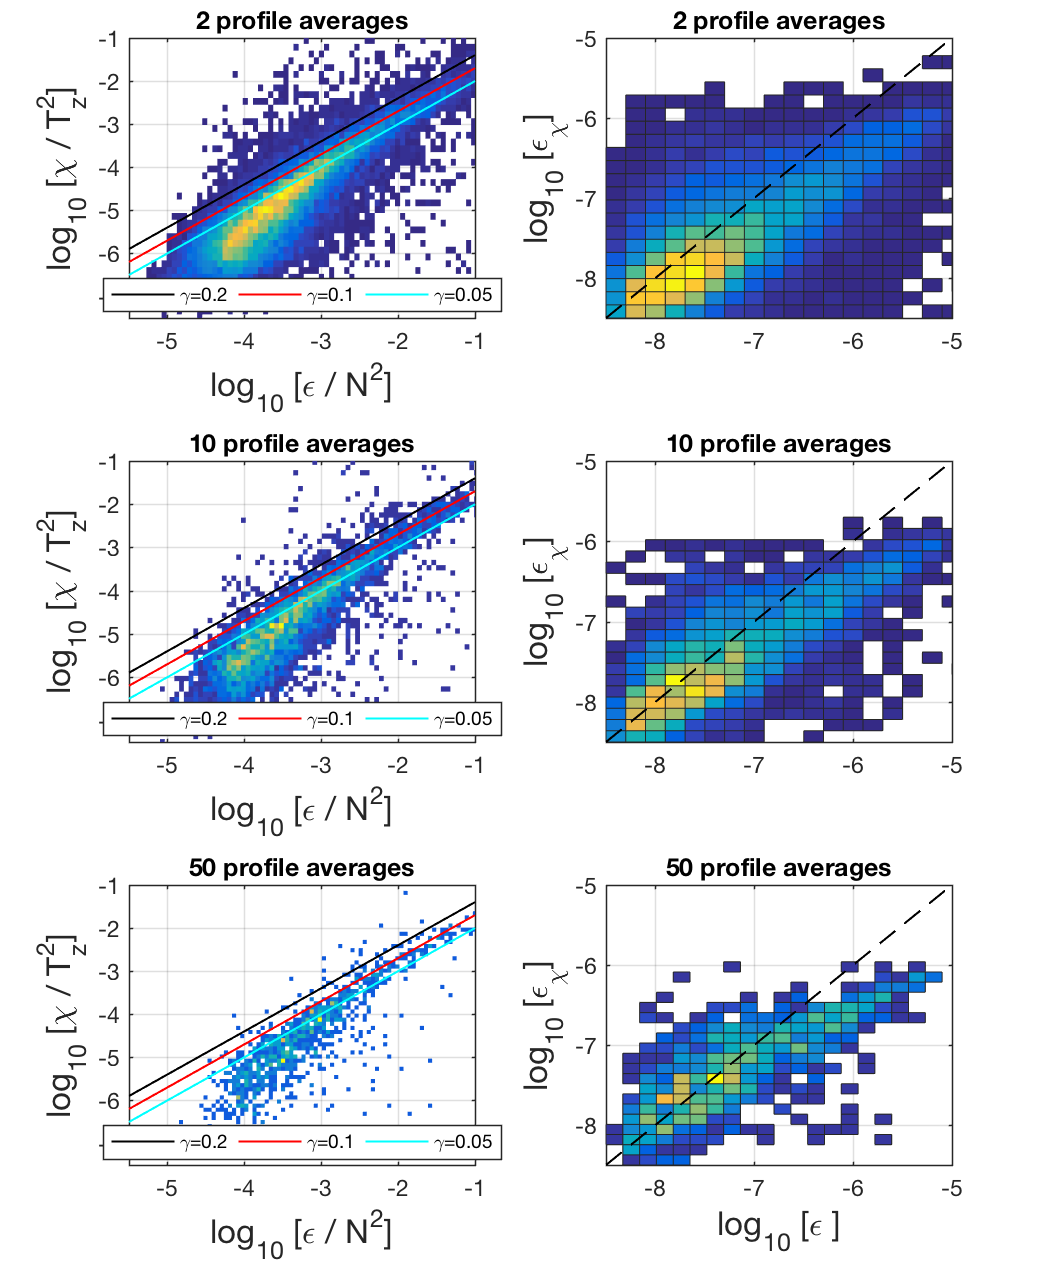
\includegraphics[scale=0.8]{eq14_NormScat_chiVscham_diff_prof_avg_screen_chi_1.png}
\caption{}
\label{}
\end{figure}

\begin{figure}[htbp]
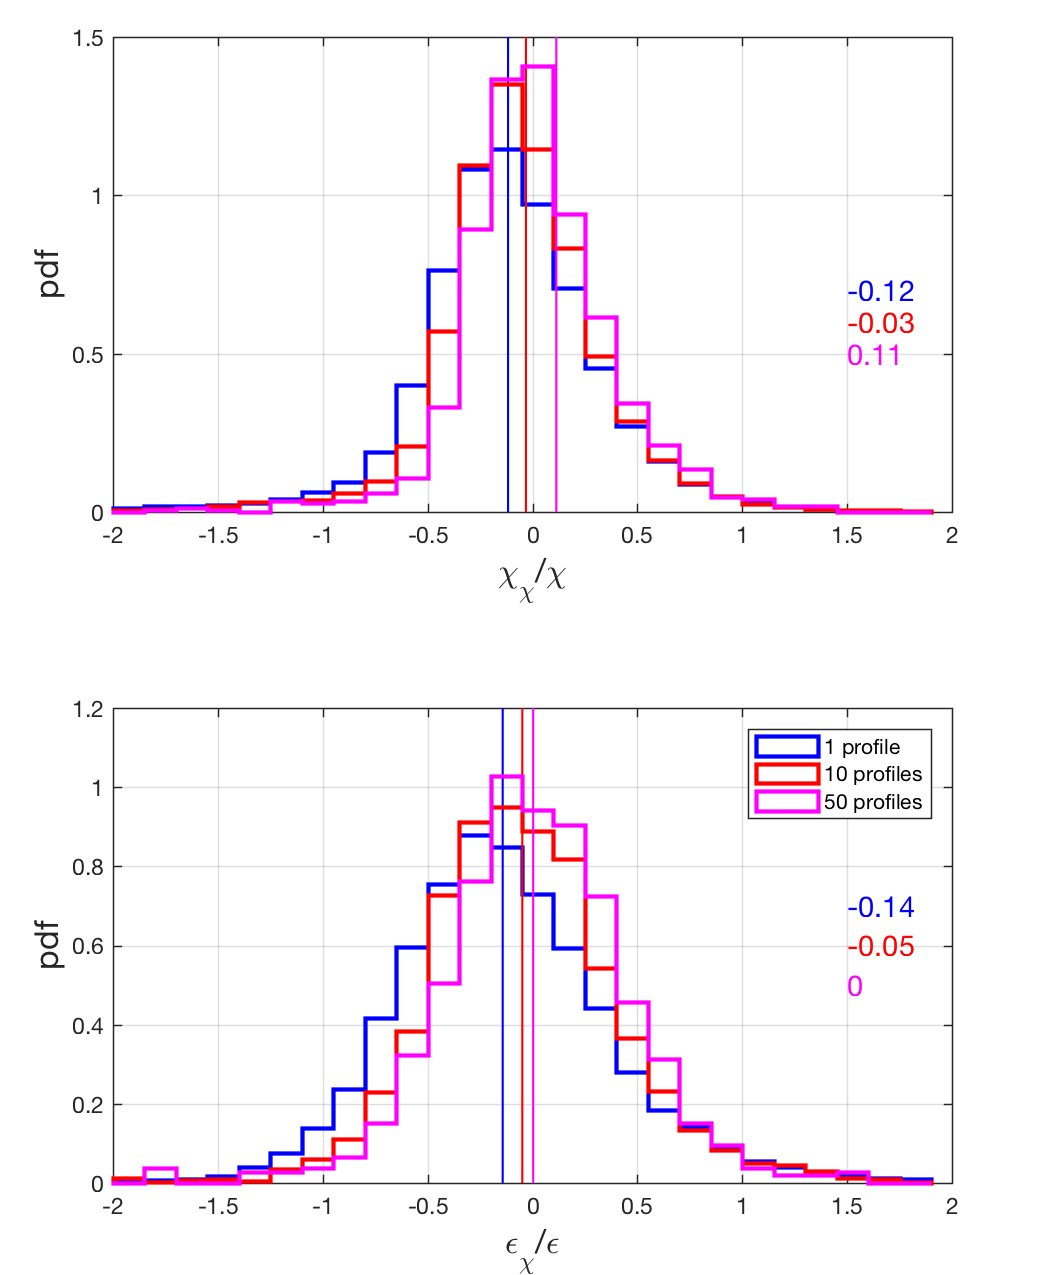
\includegraphics[scale=0.8]{eq14_eps_ratio_hist_diff_prof_avg.png}
\caption{(log10) Ratio of $\epsilon_{\chi}/\epsilon$ for different numbers of profiles averaged. Consecutive chunks of N profiles were averaged, and then (normalized) histogram of the ratios was plotted. Vertical lines are mean of $log_{10}[\epsilon_{\chi}/\epsilon]$ for each distribution. }
\label{}
\end{figure}




\clearpage
%~~~~~~~~~~~~~~~~~~~~~~~~~~~~~~~~~~~~~~~~
\section{Effects of averaging in different-sized depth bins}
%~~~~~~~~~~~~~~~~~~~~~~~~~~~~~~~~~~~~~~~~

I tried making plots of normalized chi vs eps, and scatterplots of chi-pod vs chameleon epsilon, for data averaged in different-sized depth bins (for each profile, not across profiles). They don't seem to change.

\begin{figure}[htbp]
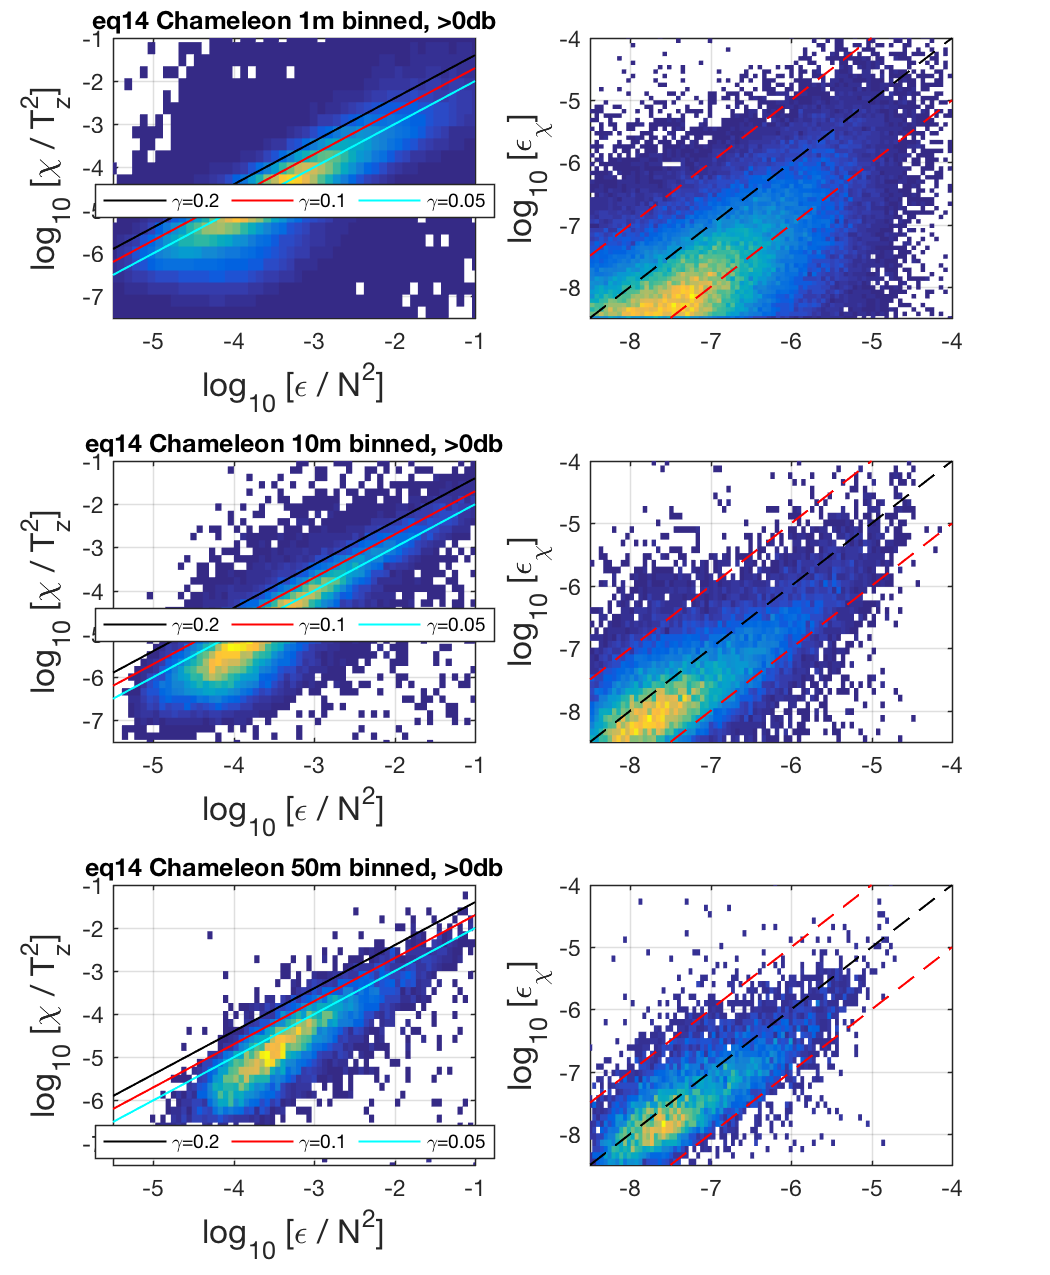
\includegraphics[scale=0.8]{eq14_NormScat_chiVscham_diff_dz_screen_chi_1.png}
\caption{Normalized plots of $\chi$ vs $\epsilon$ for different amounts of vertical averaging.}
\label{}
\end{figure}


\begin{figure}[htbp]
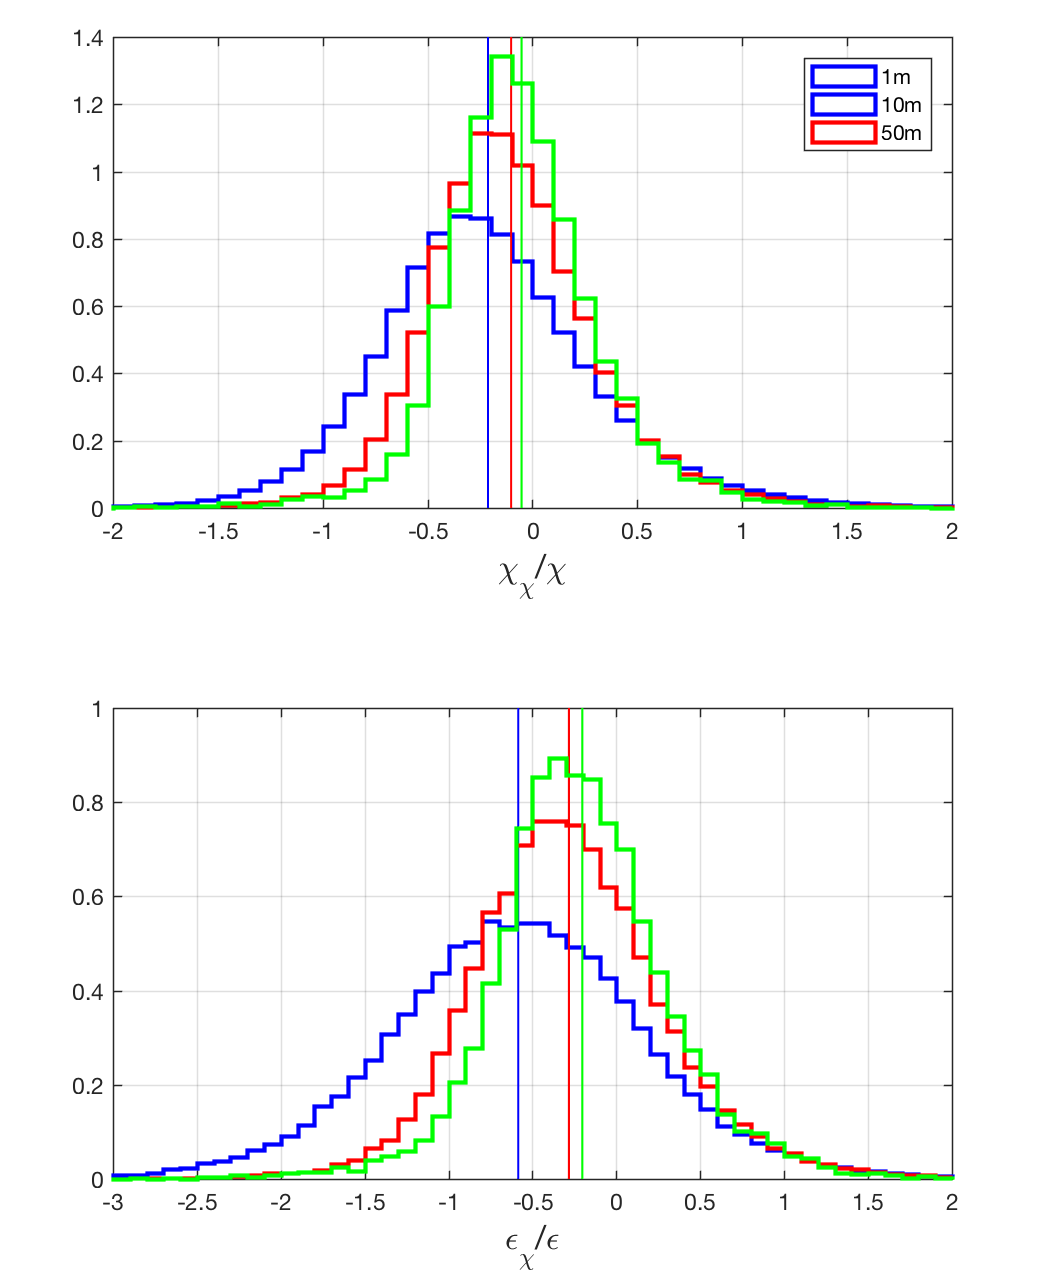
\includegraphics[scale=0.8]{eq14_chiVscham_hist_diff_dz_screen_chi_1.png}
\caption{Histogram of log10 of ratio $\epsilon_{\chi}/\epsilon$ for different amounts of vertical averaging. Vertical lines are mean of $log_{10}[\epsilon_{\chi}/\epsilon]$ for each distribution.}
\label{}
\end{figure}



%
%\clearpage
%%~~~~~~~~~~~~~~~~~~~~~~~~~~~~~~~~~~~~~~~~
%\section{Effects of averaging different numbers of profiles}
%%~~~~~~~~~~~~~~~~~~~~~~~~~~~~~~~~~~~~~~~~







\clearpage
%~~~~~~~~~~~~~~~~~~~~~~~~~~~~~~~~~~~~~~~~
\section{$\gamma$ computed from averaged quantities}
%~~~~~~~~~~~~~~~~~~~~~~~~~~~~~~~~~~~~~~~~

If we compute gamma from time-averaged $N^2,T_z,\chi,\epsilon$ do we get $\gamma=0.2$ (or a different gamma)? Estimates from the averaged data are larger (Figures \ref{gambox_eq08},\ref{gambox_eq14}) but still slightly less than 0.2 .

\begin{figure}[htbp]
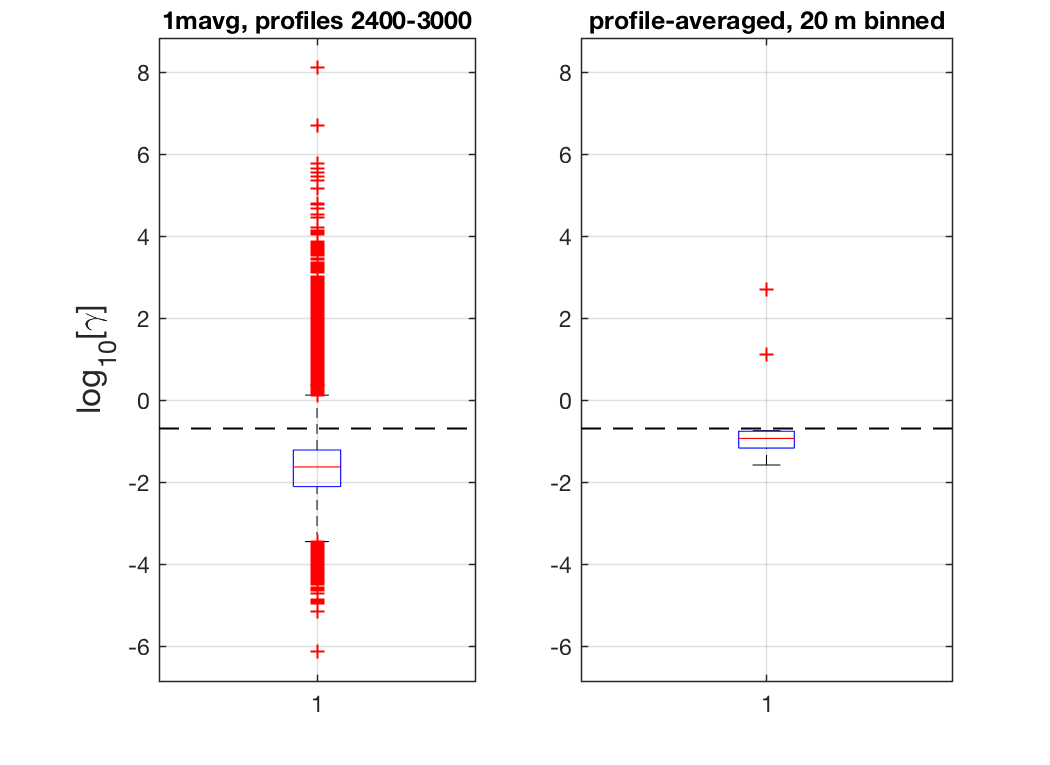
\includegraphics[scale=0.8]{eq14_gamma_point_avg_box_20mbinned.png}
\caption{Boxplots of $log_{10}[\gamma]$ for a set of profiles from EQ14. Left is for all 1m avg data. Right is for data from all profiles averaged in 10m bins. Horizontal dashed line indicates $\gamma=0.2$.}
\label{gambox_eq14}
\end{figure}



\clearpage
%~~~~~~~~~~~~~~~~~~~~~~~~~~~~~~~~~~~~~~~~
\section{Summary}
%~~~~~~~~~~~~~~~~~~~~~~~~~~~~~~~~~~~~~~~~

\begin{itemize}

\item Inidivudal (and 10m binned) $\chi$pod estimates of $\epsilon_{\chi}$ are biased low compared to Chameleon $\epsilon$.

\item This appears to be because $\gamma$ computed from the Chameleon data is lower than the assumed 0.2

\item $\gamma$ computed from averaged (across profiles) $N^2$, $T_z$, $\chi$, and $\epsilon$ is closer to 0.2

\item averaging many epsilon profiles improves comparison (if use same noise floor for epsilon as Chameleon)?

\end{itemize}

Questions:

\begin{itemize}
\item Is gamma really different here? Or is it an issue with the instrument or processing?
\item Would be good to see what gamma you get from other instruments/locations (I think Amy did this for some of the database and found gamma was about 0.2?)
\item Would be good to have 'standard' code to compute $\chi$ from thermistor data etc.? Thermistor response/noise level varies a lot though, would need a standard way to determine correction.
\end{itemize}



\end{document}  


